\documentclass[10pt]{article}

\usepackage{siunitx}
\usepackage{amsmath}
\usepackage{amsfonts}
\usepackage{booktabs}
\usepackage[margin=0.75in]{geometry}
\usepackage{graphicx}
\usepackage{mhchem}

\renewcommand{\vec}{\mathbf}
\newcommand{\R}{\mathbb{R}}


\begin{document}
  \begin{tabular}{l}
    Box Num. 33 \\
    Problem Set 35 \\
    \today
  \end{tabular}

  \begin{enumerate}
    \item \begin{enumerate}
        \item $\ce{^{27} Si} \to \ce{^{27} Al} + \ce{e^+} + \ce{v_e}$
        \item $\ce{^{74}As} \to \ce{^{74}Se} + \ce{e^-} + \overline{\ce{v_e}}$
        \item $\ce{^{228}U} \to \alpha + \ce{^{224}Th}$
        \item $\ce{^{93}Mo} + \ce{e^-} \to \ce{^{93}Nb}$
        \item $\ce{^{131}I} \to \ce{^{131}Xe} + \ce{e+} + \ce{v_e}$
    \end{enumerate}

    \item \begin{enumerate}
        \item Radioactive decay for nuclide $A$ is described by the differential equation
        \begin{equation*}
            dN_A = -N_A\lambda_A dt
        \end{equation*}
        A similar differential equation describes the decay of nuclide $B$, but the supply of nuclide $B$ is also being replenished over time:
        \begin{equation*}
            dN_B = (\lambda_A N_A - \lambda_B N_B)dt
        \end{equation*}

        \item When $B$ is stable, the differential equation is
        \begin{equation*}
            dNB_B = \lambda_A N_A dt
        \end{equation*}
        When $\lambda=\lambda_A=\lambda_B$, the differential equation is
        \begin{equation*}
            dN_B = (N_A- N_B)\lambda dt
        \end{equation*}

        \item The activity of nuclide $A$ is
        \begin{equation*}
            A_A(t) = \lambda_A N_{A,0} e^{-\lambda_A t}
        \end{equation*}
        Solving the ODE above for $N_B(t)$ gives
        \begin{equation*}
            N_B(t) = e^{-\lambda_B t} \left(
                \frac{e^{(\lambda_B-\lambda_A)t}N_{0,A}\lambda_A}{\lambda_B-\lambda_A}
            \right)
        \end{equation*}
        and the activity is
        \begin{equation*}
            A_B(t) = e^{-\lambda_B t} \lambda_B\left(
                \frac{e^{(\lambda_B-\lambda_A)t}N_{0,A}\lambda_A}{\lambda_B-\lambda_A}
            \right)
        \end{equation*}

        When $\lambda=\lambda_A=\lambda_B$,
        \begin{equation*}
            N_B(t) = N_{0,A} t \lambda e^{-\lambda t}
        \end{equation*}
        and
        \begin{equation*}
            A_B(t) = N_{0,A} t \lambda^2 e^{-\lambda t}
        \end{equation*}

        \item In the $\lambda=\lambda_A=\lambda_B$ case, we have $A_B(t) = N_{0,A} t \lambda^2 e^{-\lambda t}$. Taking the derivative,
        \begin{equation*}
            \frac{dA_B(t)}{dt} = -N_{0,A} \lambda^2 e^{-\lambda t} (\lambda  t-1)
        \end{equation*}
        This function has a maximum when $t=1/\lambda$. The maximum is $A_B = N_{0,A}\lambda/e$.

        \item

        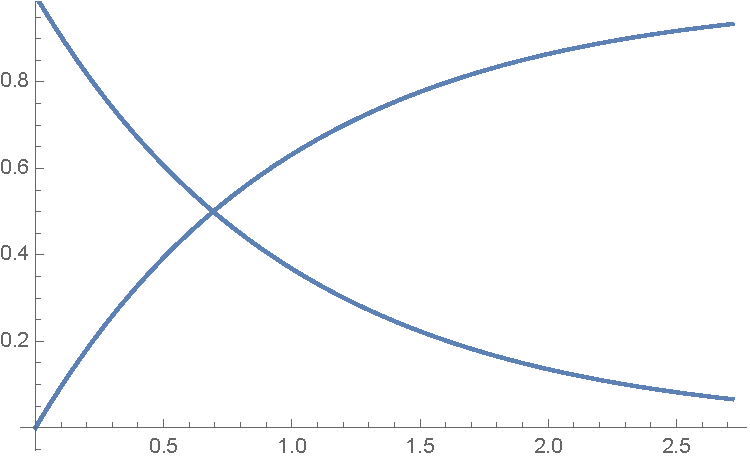
\includegraphics[width=0.6\textwidth]{2eplot}

        \item

        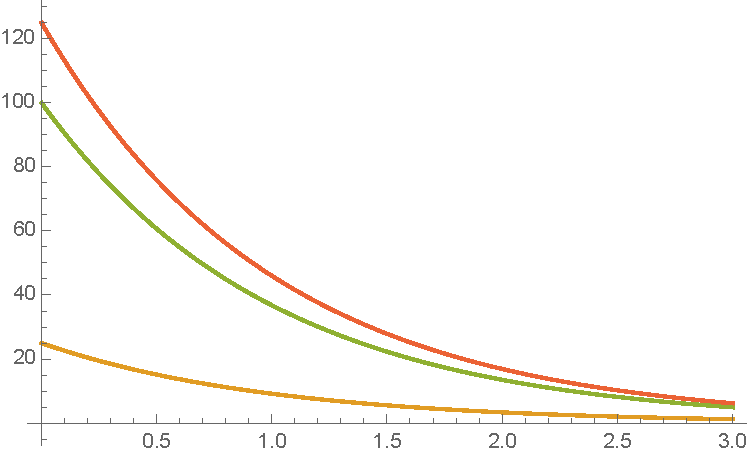
\includegraphics[width=0.6\textwidth]{2fplot}
    \end{enumerate}

    \item \begin{enumerate}
        \item The atomic mass of \ce{^{149}Eu} is $148.917931238u$, which is smaller than the mass of \ce{^{149}Gd}, so $\beta^-$ decay is not energetically favorable. An alpha decay would result in a total product mass of $148.915352277$, so this is (barely) energetically favorable. A $\beta^+$/neutron capture reaction would result in a product mass of $148.917184735$u, so this reaction is also favorable.

        \item \ce{^{151}Eu} is stable. All of the potential decay products ($\ce{^{147}Pm}+\alpha$, \ce{^{151}Gd}, and \ce{^{151}Sm}) have a higher mass.

        \item \ce{^{152}Eu} decays via $\beta^+$ and $\beta^-$ decays. The products of these reactions, \ce{^{152}Gd} and \ce{^{152}Sm}, both have lower masses than \ce{^{152}Eu}, making this reaction energetically favorable.

        \item The only decay mode this isotope can undergo is $\beta^-$. Alpha decay results in \ce{^{155}Pm} and an alpha particle, which together have a higher mass than the original. Only $\beta^-$ decay results in a decrease in energy.
    \end{enumerate}

    \item \begin{enumerate}
        \item This reaction is endothermic, with a threshold energy of $0.0045267uc^2 = \SI{4.2}{\mega\electronvolt}$.

        \item This reaction is exothermic.

        \item This reaction is exothermic.

        \item This reaction is endothermic, with a threshold energy of $0.005368007uc^2 = \SI{5}{\mega\electronvolt}$.
    \end{enumerate}

  \end{enumerate}


\end{document}
